
\begin{frame}{Forskjeller i bildeprotokoller}
    \begin{tikzpicture}
        \node[draw=black] at (-7, -3.25) {};
        \node[draw=black] at (7, 3.25) {};

        \only<1>{
            \mriside{-4.5}{-0.2175}{1.5cm}{data/mri_sagittal.png}
        }
        \only<2>{
            \mriside{-4.5}{-0.2175}{1.5cm}{data/mri_low_quality.png}
        }
        \only<3>{
            \mriside{-4.5}{-0.2175}{1.5cm}{data/t2.png}
        }
        \only<1-3>{
            \cnnarrow{(input.east)}{($ (input.center) + (3, 0) $)}{black}
            \cnn{-2.7}{-0.2175}{0.1}{0.15}{uiogreen}{1}
            \node[anchor=west, align=left, font=\normalfont\linespread{0.9}\selectfont] (output1) at ($ (3.55, -0.2175) + (0, 0.5) $) {Pasient};
            \node[anchor=west, align=left, font=\normalfont\linespread{0.9}\selectfont] (output2) at ($ (3.55, -0.2175) - (0, 0.5) $) {Frisk\\kontroll};
            \cnnarrow{($ (output1.west) - (1, 0.5) $)}{($ (output1.west) + (0.1, 0) $)}{black}
            \cnnarrow{($ (output2.west) - (1, -0.5) $)}{($ (output2.west) + (0.1, 0) $)}{black}
        }
        \only<4-8>{
            \node[anchor=south, font=\tiny, text width=10.5cm, align=flush center] at (0, -3.4) {
                Juan E. Iglesias et al., SynthSR: A public AI tool to turn heterogeneous clinical brain scans into high-resolution T1-weighted images for 3D morphometry. \textit{Science Advances} (2023)
            };
        }
        \only<4-7>{
            \mriside[low]{-5.5}{-0.2175}{1.5cm}{data/mri_low_quality.png}
            \only<6-7>{
                \cnnarrow{(low.east)}{($ (low.center) + (3, 0) $)}{black}
                \unet{-3.5}{-0.2175}{0.05}{0.15}{uiogreen}{1}
                \cnnarrow{($ (low.east) + (7.46, 0) $)}{($ (low.east) + (9.48, 0) $)}{black}
            }
            \mriside[high]{5.5}{-0.2175}{1.5cm}{data/mri_sagittal.png}
            \only<5-6>{
                \node[rounded corners=0.05cm, fill=black!70, text=white] (distortion) at (0, 2.5) {Degradering};
                \begin{scope}[transparency group, opacity=0.5]
                    \draw[-stealth, line width=2pt, black] (high) |- (distortion);
                    \draw[-stealth, line width=2pt, black] (distortion) -| (low);
                \end{scope}
            }
        }
        \only<8>{
            \node[inner sep=0pt, draw=black] at (0, 0.5) {
                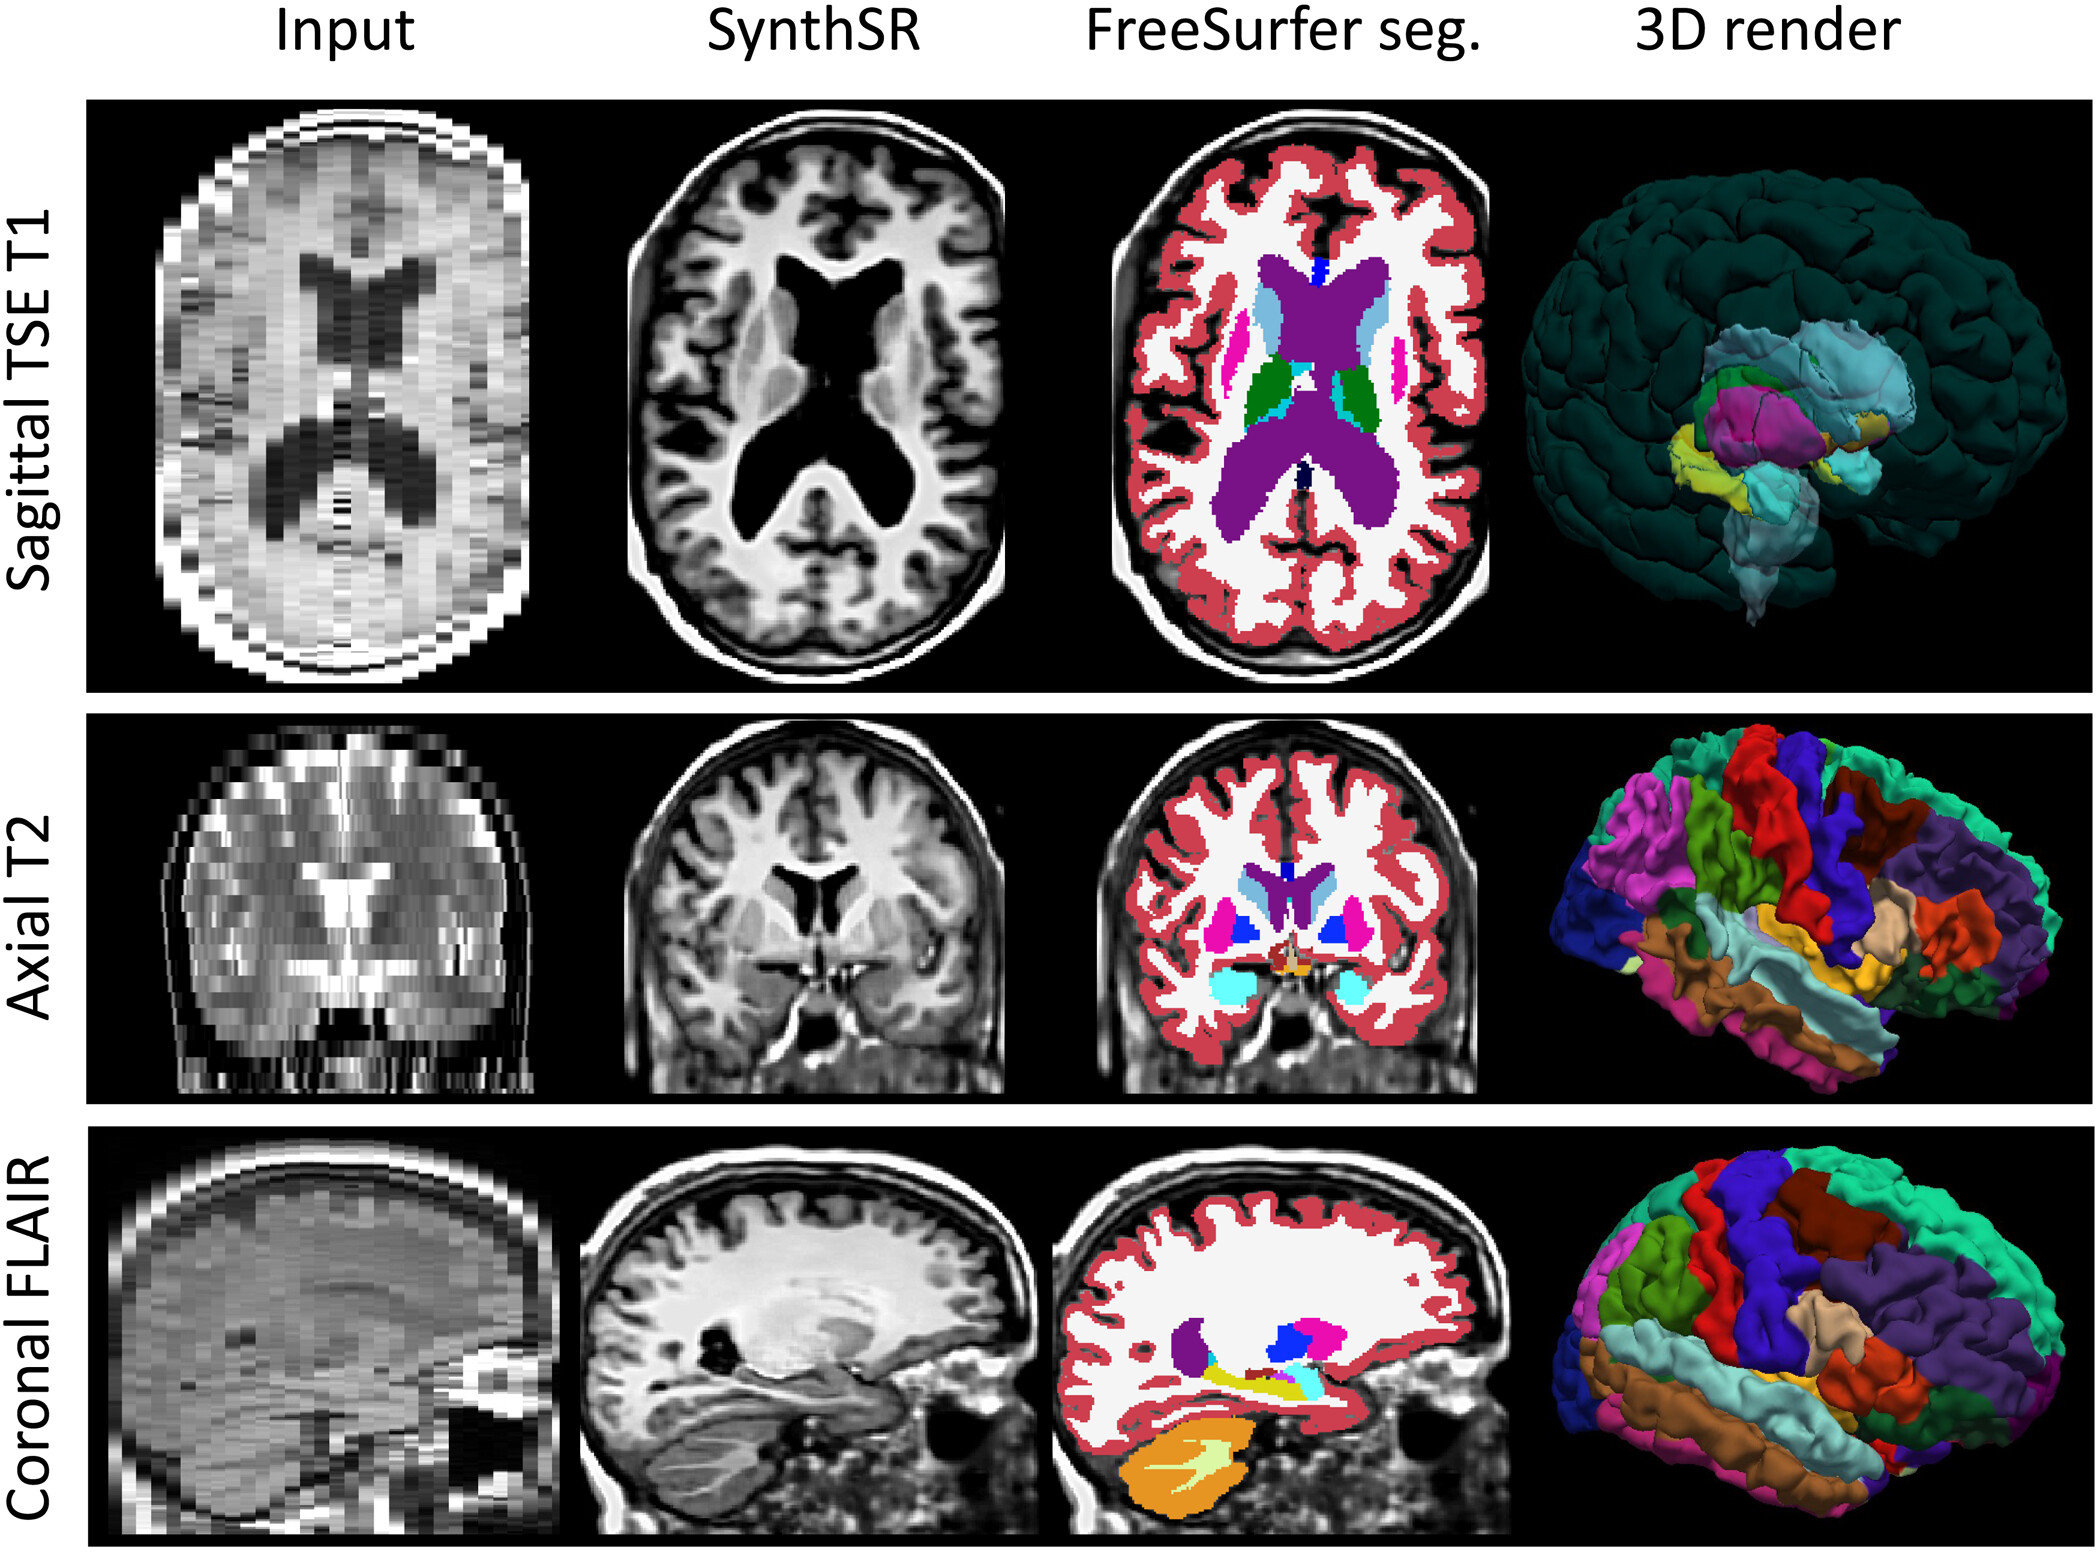
\includegraphics[width=7cm]{data/synthsr.jpg}
            };
        }
        \only<9-10>{
            \mriside[high]{-5.9}{1.0825}{1.5cm}{data/mri_sagittal.png}
            \node[font=\footnotesize\linespread{0.9}\selectfont, align=center, anchor=south] at ($ (high.north) + (0, 0.3) $) {Forskningsdata};
            \cnnarrow{(high.east)}{($ (high.center) + (5.5, -1.3) $)}{black}

            \only<10>{
                \mriside[low]{-5.9}{-1.5125}{1.5cm}{data/mri_low_quality.png}
                \node[font=\footnotesize\linespread{0.9}\selectfont, align=center, anchor=north] at ($ (low.south) - (0, 0.3) $) {Klinisk data};
                \node[rounded corners=0.05cm, fill=black!70, text=white] (synthsr) at ($ (low) + (2.5, 0) $) {SynthSR};
                \cnnarrow{(low.east)}{(synthsr)}{black}
                \cnnarrow{(synthsr)}{($ (low.center) + (5.5, 1.3) $)}{black}
            }

            \cnn{-1}{-0.2175}{0.1}{0.15}{uiogreen}{1}
            \node[font=\small\linespread{0.9}\selectfont, anchor=east, align=left] (output) at (7, -0.2175) {Klinisk\\prediksjon};
            \cnnarrow{($ (-1, -0.2175) + (5.25, 0) $)}{(output)}{black}
        }
        \only<11>{
            \mriside[high]{-3}{0}{3cm}{data/mri_low_quality.png}
            \mriside[high]{3}{0}{3cm}{data/mri_sagittal.png}
        }
        \only<12>{
            Brain age offset
        };
    \end{tikzpicture}
\end{frame}